\documentclass[../main-sheet.tex]{subfiles}
\usepackage{../style}
\graphicspath{ {../img/} }
\backgroundsetup{contents={}}
% \DeclareUnicodeCharacter{2212}{-}
\begin{document}
\chapter{Power Series Solutions to the Legendre Equation}
\section{The Legendre equation}
The equation
\begin{equation}
    \left(1 - x^2\right)y'' - 2xy' + \alpha(\alpha + 1)y = 0, \label{eq:legen}
\end{equation}
where $ \alpha $ is any real constant, is called Legendre's equation.
When $ \alpha\in\mathbb{Z}^{+}$, the equation has polynomial solutions called
Legendre polynomials. In fact, these are the same polynomial that encountered earlier in connection with the Gram-Schmidt process.\\
The equation \eqref{eq:legen} can be rewritten as
\[
    \left[\left(x^2 - 1\right)y'\right]' = \alpha(\alpha + 1)y,
\]
which has the form $ T (y) = \lambda y $, where $ T (f ) = (pf')'t' $, with
$ p(x ) = x^2 - 1 $ and $ \lambda = \alpha(\alpha + 1) $.
\begin{note}
    The nonzero solutions of \eqref{eq:legen} are eigenfunctions of $ T $
    corresponding to the eigenvalue $ \alpha(\alpha + 1). $
\end{note}

Since $ p(1) = p( 1) = 0 $, $ T $ is symmetric with respect to the inner product
\[
    (f,g) =\int_{-1}^1 f (x )g (x )\dx.
\]

Thus, eigenfunctions belonging to distinct eigenvalues are orthogonal.
% \newpage
\section{Power series solution for the Legendre equation}
The Legendre equation can be put in the form
\[
    y'' + p(x )y' + q(x )y = 0,
\]
where
\[
    p(x) =\frac{2x}{1-x^2}\, \text{ and }\, q(x ) =\frac{\alpha(\alpha + 1)}{1-x^2}\, \text{ if }\, x^2\neq 1
\]
 
Since $\frac{1}{1-x^2}=\sum_{n=0}^\infty x^{2n}  $ for $ \abs{x} < 1 $, both $ p(x ) $ and $ q(x ) $ have power series expansions in the open interval $ (-1, 1) $.\\
Thus, seek a power series solution of the form
\[
    y (x ) =\sum_{n=0}^\infty	a_n x^n,\, x \in (-1, 1).
\]
Differentiating term by term, we obtain
\[
    y'(x ) = \sum_{n=1}^\infty n a_n x^n-1 \, \text{ and}\, y'' =\sum_{n=2}^\infty n(n - 1)a_nx^{n-2}.
\]
Thus,
\[
    2xy'= \sum_{n=1}^\infty 2na_nx^n = \sum_{n=0}^\infty 2na_nx^n
\]
and
\begin{align*}
    (1 - x^2)y''&=\sum_{n=2}^\infty n(n - 1)a_nx^{n-2} - \sum_{n=2}^\infty n(n - 1)a_nx^n\\
    &=\sum_{n=0}^\infty (n + 2)(n + 1)a_{n+2}x_n - \sum_{n=0}^\infty n(n - 1)a_nx^n\\
    &=\sum_{n=0}^\infty \left[(n + 2)(n + 1)a_{n+2} - n(n - 1)a_n\right]xn
\end{align*}
Substituting in \eqref{eq:legen}, we obtain
\[
    (n +2)(n +1)a_{n+2} -n(n-1)a_n -2na_n +\alpha(\alpha+1)a_n = 0, n \geq 0, 
\]
which leads to a recurrence relation
\[
    a_{n+2}=-\frac{(\alpha-n)(\alpha+n+1)}{(n+1)(n+2)}a_n
\]
Thus, we obtain
\begin{align*}
    a2	&=-\frac{\alpha(\alpha+1)}{1\cdot 2}a_0\\
    a_4&=-\frac{(\alpha-2)(\alpha + 3)}{3\cdot4}=(-1)^2\frac{\alpha(\alpha-2)(\alpha + 1)(\alpha + 3)}{4!}a_0\\
    &\vdots\\
    a_{2n}&=(-1)^n\frac{\alpha(\alpha - 2)\dots (\alpha - 2n + 2) \cdot (\alpha + 1)(\alpha + 3) \dots (\alpha + 2n - 1)}{(2n)!}a_0
\end{align*}
Similarly, we can compute $ a_3, a_5, a_7,\dots, $ in terms of $ a_1 $ and obtain
\begin{align*}
    a_3&=\frac{(\alpha-1)(\alpha + 2)}{2\cdot3}a_1\\
    a_5&=-\frac{(\alpha-3)(\alpha + 4)}{4\cdot5}a_3=(-1)^2\frac{(\alpha-1)(\alpha-3)(\alpha + 2)(\alpha + 4)}{5!}a_1\\
    &\vdots\\
    a_{2n+1}&=(-1)^n\frac{(\alpha-1)(\alpha-3)\dots(\alpha - 2n + 1)(\alpha + 2)(\alpha + 4)\dots(\alpha + 2n)}{(2n + 1)!}a_1
\end{align*}
Therefore, the series for $ y (x ) $ can be written as
\[
    y (x ) = a_0y_1(x ) + a_1y_2(x ),
\]
where,
\begin{align*}
    y1(x ) &= 1 +\sum_{n=0}^\infty(-1)^n\frac{\alpha(\alpha-2)\dots(\alpha-2n+2)\cdot(\alpha+1)(\alpha+3)\dots(\alpha+2n-1)}{(2n)!}x^{2n},\text{ and}\\ 
    y2(x ) &= x + \sum_{n=0}^\infty(-1)^n\frac{(\alpha-1)(\alpha-3)\dots(\alpha-2n+1)\cdot(\alpha+2)(\alpha+4)\dots(\alpha+2n)}{(2n+1)!}x^{2n+1}
\end{align*}
\begin{note}
    The ratio test shows that $ y_1(x ) $ and $ y_2(x ) $ converges for $ \abs{x} < 1 $. These solutions $ y_1(x ) $ and $ y_2(x ) $ satisfy the initial conditions
    \[
        y_1(0) = 1,\, y_1' (0) = 0, \,y_2(0) = 0, y_2' (0) = 1.
        \]
    Since $ y_1(x ) $ and $  y2(x ) $ are independent, the general solution of the Legendre equation over $ (-1, 1) $ is
    \[
        y (x ) = a_0y_1(x ) + a_1y_2(x ) 
    \]
    with arbitrary constants $ a_0 $ and $ a_1 $.
\end{note}
\subsection{Observations}
    \emph{Case I.}\\
    When $ \alpha = 0 $ or $ \alpha = 2m $, we note that
    \[
        \alpha(\alpha - 2)\dots(\alpha - 2n + 2) = 2m(2m - 2)\dots(2m - 2n + 2) = \frac{2^n\,m!}{(m - n)!}
    \]
    and
    \[
        (\alpha + 1)(\alpha + 3)\dots(\alpha + 2n - 1)   =   (2m + 1)(2m + 3)\dots(2m + 2n - 1)=\frac{(2m + 2n)!\,m!}{2^n (2m)!(m + n)!}
    \]
    Then, in this case, $ y_1(x ) $ becomes
    \[
        y_1(x ) = 1 +\frac{(m!)^2}{(2m)!}\sum_{k=0}^m (-1)^k\frac{(2m+2k)!}{(m-k)!\,(m+k)!\,(2k)!}x^{2k}
    \]
    which is a polynomial of degree $ 2m $. In particular, for $ \alpha = 0, 2, 4(m = 0, 1, 2) $, the corresponding polynomials are
    \[
        y_1 (x ) = 1,\,  1 - 3x^2  ,  1 - 10x^2+\frac{35}{3}x^4
    \]
    Note that the series $ y_2(x ) $ is not a polynomial when $ \alpha $ is even because the coefficients of $ x^{2n+1} $ is never zero.\\
    \emph{Case II.}\\
    When $ \alpha = 2m + 1,\, y_2(x ) $ becomes a polynomial and $ y_1(x ) $ is not a polynomial.\\
    In this case,
    \[
        y_2(x)=x+\frac{(m!)^2}{(2m+1)!}\sum_{k=0}^m (-1)^k\frac{(2m+2k+1)!}{(m-k)!\,(m+k)!\,(2k+1)!}x^{2k+1}
    \]
    For example, when $ \alpha = 1, 3, 5 (m = 0, 1, 2) $, the corresponding polynomials are
    \[
        y_2(x ) = x, x - \frac{5}{3}x^3, x -\frac{14}{3}x^3 +\frac{21}{5}x^5
    \]
\section{The Legendre polynomial}
Let,
\begin{equation}
    P_n(x )=\frac{1}{2^n}\sum_{r=0}^{[n/2]}\frac{(-1)^r (2n - 2r )!}{r !(n - r )!(n - 2r )!}x^{n-2r} \label{eq:2}
\end{equation}
where $ [n/2] $ denotes the greatest integer $ \leq n/2. $
\begin{itemize}
    \item When $ n $ is even, it is a constant multiple of the polynomial $ y1(x ) $.
    \item When $ n $ is odd, it is a constant multiple of the polynomial
    $ y2(x ) $.
\end{itemize}
The first five Legendre polynomials are
\[
    P_0(x ) = 1,\; P_1(x ) = x,\;P_2(x ) =\frac{1}{2}\left(3x^2 - 1\right),\; P_3(x)=\frac{1}{2}\left( 5x^3-3x \right)
\]
\[
    P_4(x ) =\frac{1}{8}\left(35x^4 - 30x^2 + 3\right),\,P_5(x ) =\frac{1}{8}\left(63x^5 - 70x^3 + 15x \right)
\]
\begin{figure}[H]
    \centering
    \import{../tikz/}{leg.tikz}
    % 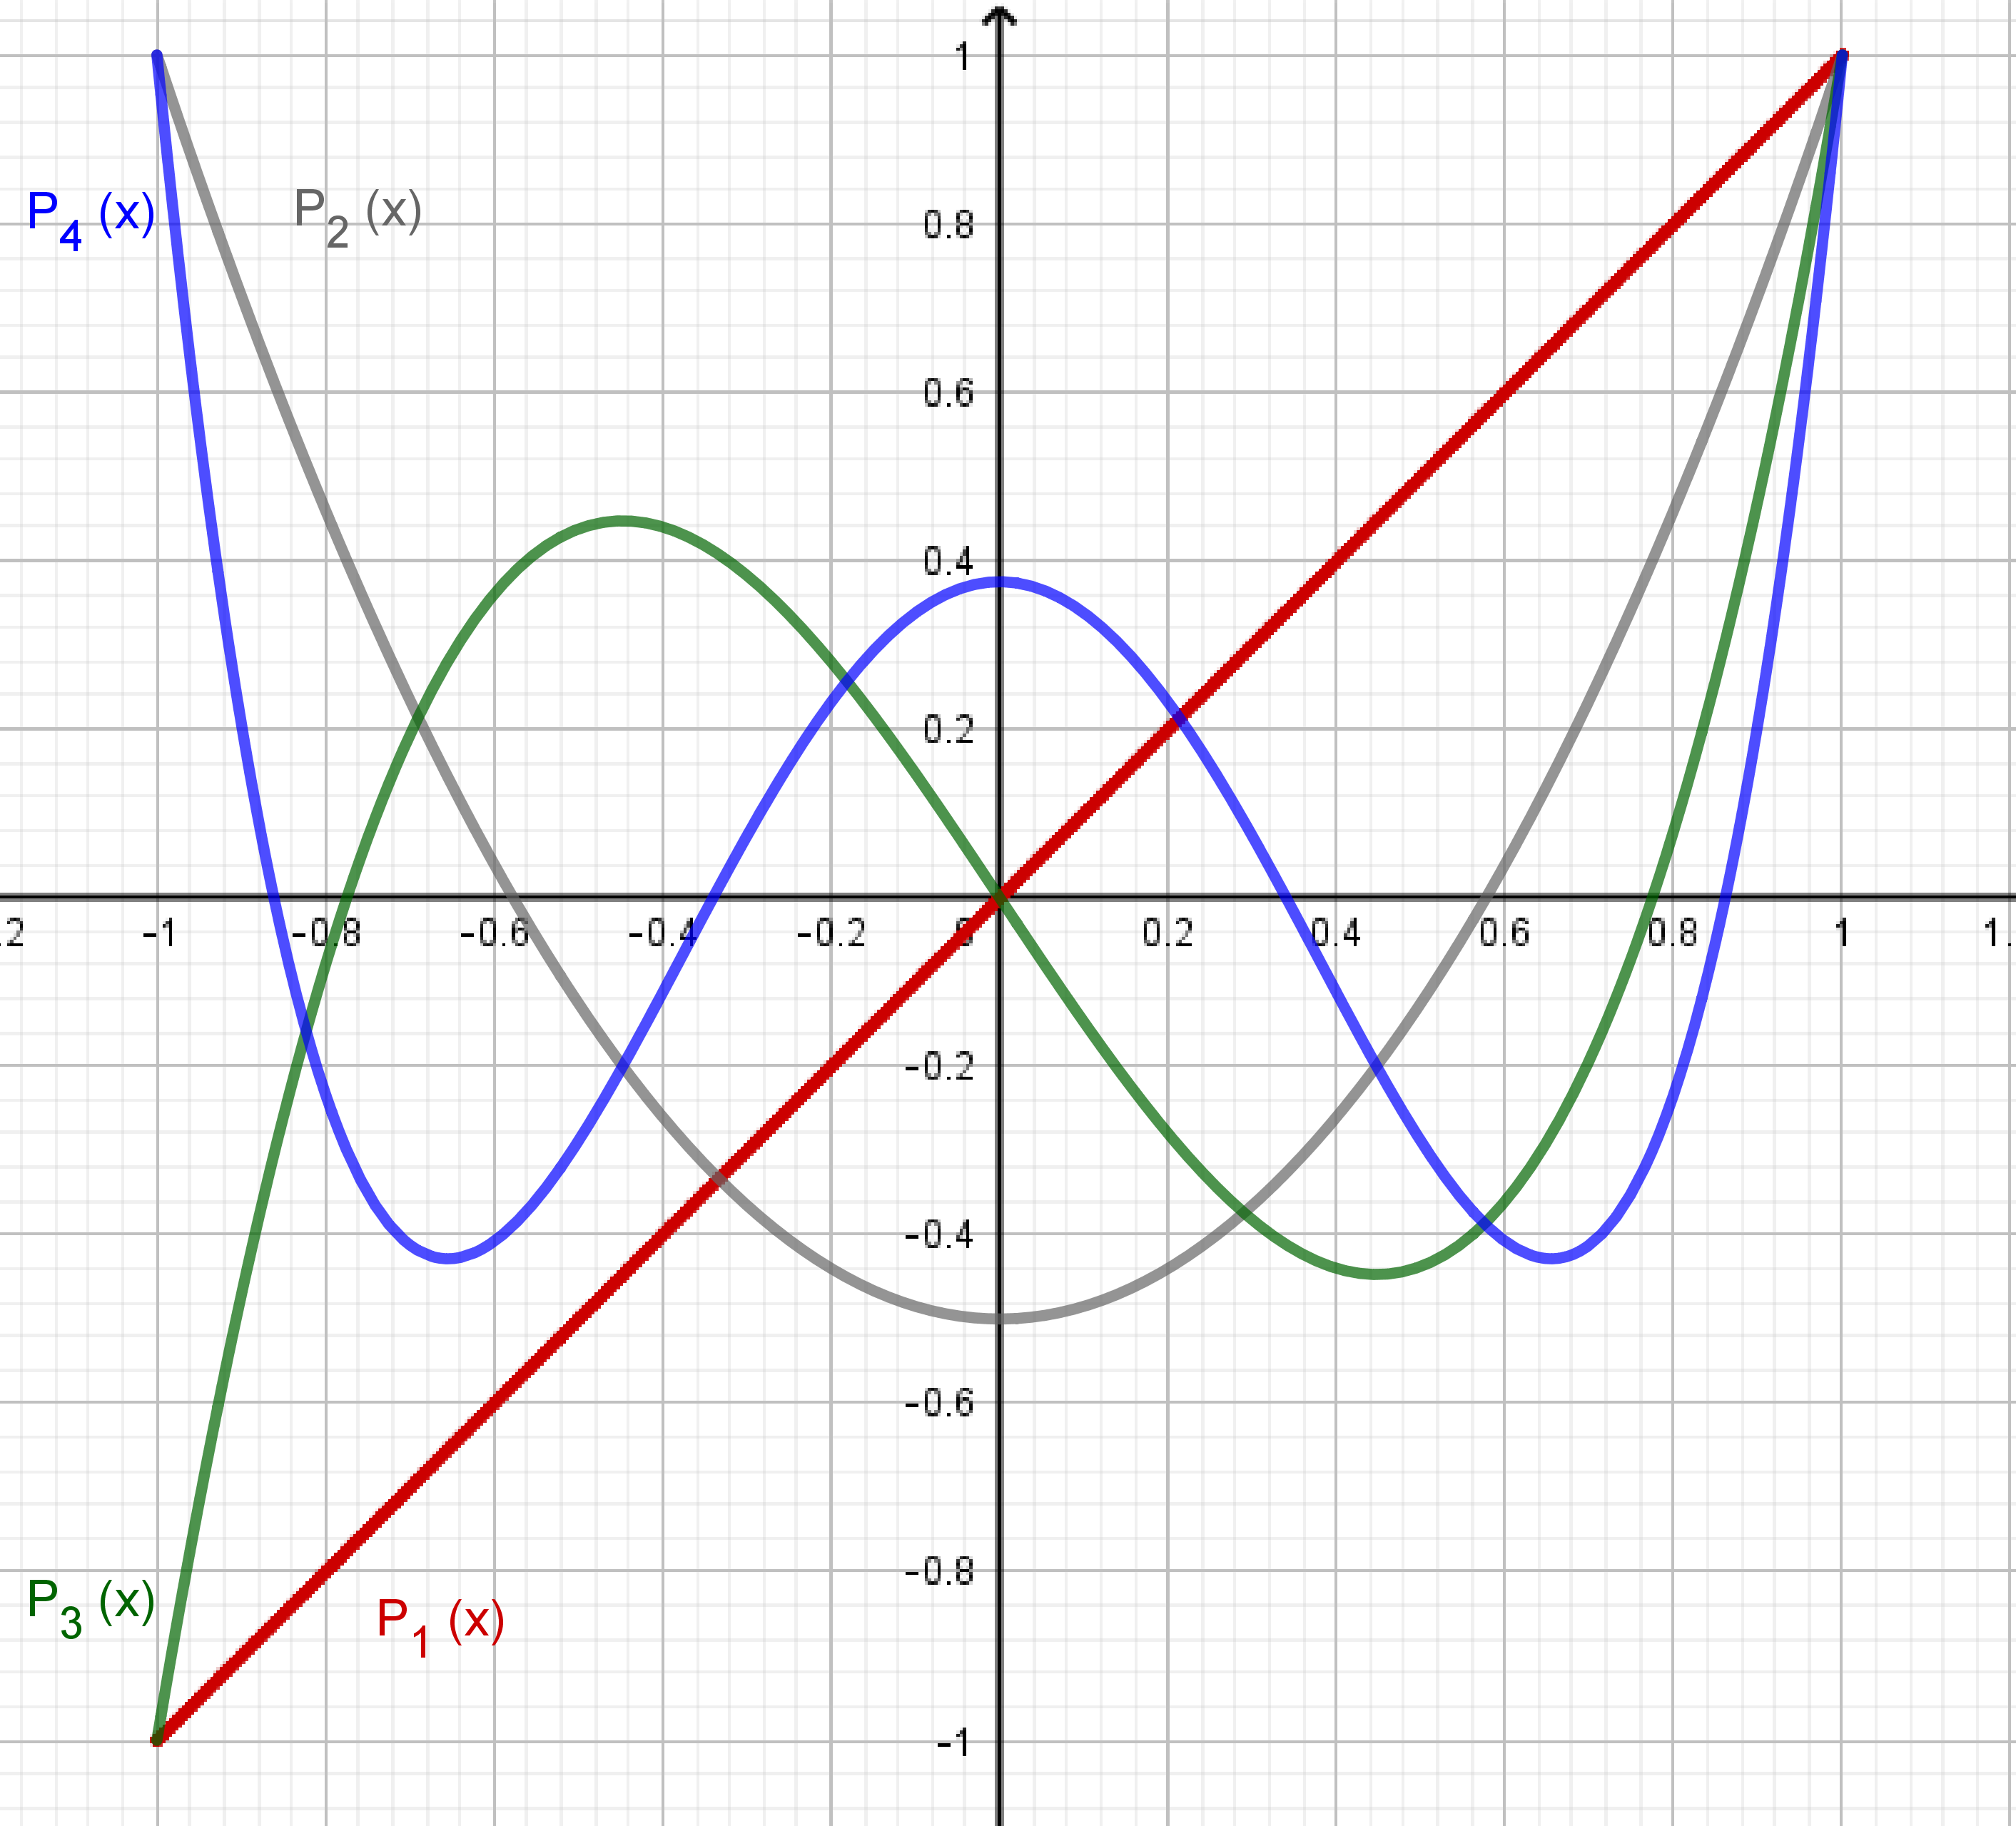
\includegraphics[scale=.25]{legendre.png}
    \caption{Legendre polynomial $ (P_0(x),P_1(x),P_2(x),P_3(x),P_4(x),P_5(x)) $ over the interval $ [-1, 1] $}
\end{figure}
% \newpage
\section{Rodrigues's formula for the Legendre polynomials}
Note that
\[
    \frac{(2n - 2r )!}{(n-2r)!}x^{n-2r}=\ddxn{}{n}x^{2n-2r}\,\text{ and } \frac{1}{r!\,(n - r )!}=\frac{1}{n!}\binom{n}{r}
\]
Thus,$  P_n(x ) $ in \eqref{eq:2} can be expressed as
\[
    P_n(x ) =\frac{1}{2^n\,n!}\ddxn{}{n}\sum_{r=0}^{[n/2]}(-1)^r\binom{n}{r}x^{2n-2r}
\]
When $ [n/2] < r\leq n $, the term $ x^{2n-2r}  $ has degree less than $ n $, so its $ n $th derivative is zero. This gives
\[
    P_n(x ) =\frac{1}{2^n\,n!}\ddxn{}{n}\sum_{r=0}^{n}(-1)^r\binom{n}{r}x^{2n-2r}=\frac{1}{2^n\,n!}\ddxn{}{n}\left( x^2-1 \right)^n
\]
which is known as Rodrigues' formula.
\section{Properties of the Legendre polynomials $ P_n(x) $}
\begin{itemize}
    \item For each $ n\geq 0 $, $ P_n(1) = 1 $. Moreover, $ P_n(x ) $ is the only polynomial which satisfies the Legendre equation
        \[
            \left(1 - x^2\right)y'' - 2xy' + n(n + 1)y = 0
        \]
    and $  Pn(1) = 1 $.
    \item For each $ n \geq 0 $, $ P_n(-x ) = (-1)^n P_n(x ) $.
    \item 
        \[
            \int_{-1}^1 P_n(x)P_m(x)=
            \begin{cases}
                \,\,0&\text{if }m\neq n\\
                \frac{2}{2n+1}&\text{if }m=n
            \end{cases}
        \]
    \item If $ f (x ) $ is a polynomial of degree $ n $, we have
        \[
            f (x ) =\sum_{k=0}^n c_k P_k (x ), \text{ where}
        \]
        \[
            c_k=\frac{2k + 1}{2}\int_{-1}^1 f(x)P_k(x)\dx
        \]
    \item It follows from the orthogonality relation that
        \[
            \int_{-1}^1 g(x)P_n(x)\dx=0
        \]
        for every polynomial $ g (x ) $ with deg$ (g (x )) < n $.
\end{itemize}
\end{document}